\section{When the loss lies}
\label{sec:collapse}

We trained a few dozen models with the objective of \cref{sec:objective}, and some failed in ways the loss did not show. This section describes the two failure modes (\cref{fig:anatomy}), explains why the usual health signals miss them and defines the monitor we now rely on.

\begin{figure*}[t]
  \centering
  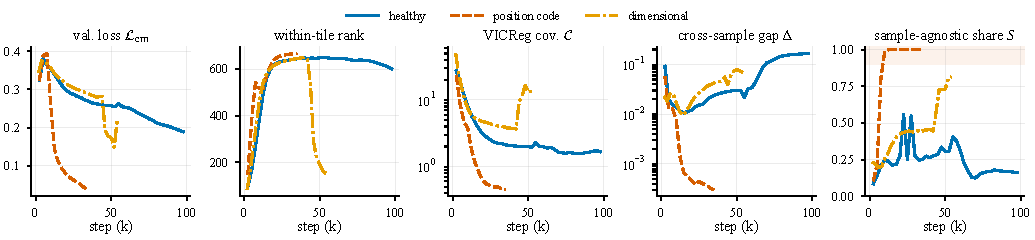
\includegraphics[width=\textwidth]{figures/anatomy.pdf}
  \caption{A healthy run, a position-code collapse and a dimensional collapse (validation curves of runs A1, B1 and D1 in \cref{tab:supp_runs}, which use different recipes). During the position code the loss falls tenfold, the within-tile rank rises and the VICReg covariance drops, all apparent improvements, while the cross-sample gap $\Delta$ goes to zero. In the dimensional collapse the rank falls and the covariance rises, but $\Delta$ increases. Only $S$ (\cref{eq:share}) rises in both; the band marks $S{>}0.9$.}
  \label{fig:anatomy}
\end{figure*}

\subsection{Two failure modes}

\paragraph{Dimensional collapse.} In the run of \cref{fig:anatomy} (fixed-GSD stems, seven products, peak learning rate $10^{-4}$), the effective rank of the target tokens within a tile fell from 651 to 163 between 40k and 52k steps. The VICReg covariance rose from 3.7 to 13.6, the expert load drifted out of balance, and the median gradient norm went from 0.05 to over 200. The validation loss kept falling, from 0.280 to 0.149. This is the dimensional collapse known from joint-embedding methods~\cite{jing2022understanding,hua2021feature}: per-feature variance survives, but the representation concentrates in a few directions. Four of our runs failed this way (\cref{tab:signals}).

\paragraph{Position-code collapse.} The second mode is harder to see. Between 5k and 35k steps of the run in \cref{fig:anatomy}, the validation loss fell from 0.389 to 0.038, the within-tile rank of targets and predictions rose from 382 to 667 and from 160 to 632, and the covariance penalty fell from 8.5 to 0.45. Yet the prediction for a footprint ended with cosine 0.972 to its own target and 0.971 to the target of another footprint. At every cell the model emitted a vector that depended on the cell's position and hardly at all on the terrain. None of its low loss came from content, and every standard signal said the run had improved. Three runs ended this way (\cref{tab:signals}).

\begin{table*}[t]
  \centering
  \small
  \setlength{\tabcolsep}{3.6pt}
  \caption{Common signals while a run fails (runs B1, B2, C2, D1--D3 and E1 in \cref{tab:supp_runs}), from the last healthy validation to the end of the failure. Rank: effective rank of the target tokens within one tile. Colors show what a practitioner would read into each change (\textcolor{ForestGreen}{looks better}, \textcolor{BrickRed}{looks worse}). Only $S$ moves the same, correct way in all seven.}
  \label{tab:signals}
  \begin{tabular}{@{}llccccccc@{}}
    \toprule
    Run & Mode & Steps & Val.\ loss $\mathcal{L}_{\text{cm}}$ & Within-tile rank & VICReg $\mathcal{C}$ & Gap $\Delta$ & Share $S$ \\
    \midrule
    Long-short attention~\cite{zhu2021long} & position    & 5k$\to$35k    & \textcolor{ForestGreen}{.389$\to$.038} & \textcolor{ForestGreen}{382$\to$667} & \textcolor{ForestGreen}{8.5$\to$0.45} & \textcolor{BrickRed}{.013$\to$.0003} & \textcolor{BrickRed}{.22$\to$1.00} \\
    \quad + border clamp                    & position    & 5k$\to$60k    & \textcolor{ForestGreen}{.393$\to$.030} & \textcolor{ForestGreen}{369$\to$665} & \textcolor{ForestGreen}{8.0$\to$0.44} & \textcolor{BrickRed}{.017$\to$.0003} & \textcolor{BrickRed}{.36$\to$1.00} \\
    Standard attn., $w_c{=}0.05$            & position    & 1k$\to$8.5k   & .423$\to$.429                          & \textcolor{ForestGreen}{262$\to$505} & \textcolor{ForestGreen}{3.2$\to$0.26} & \textcolor{BrickRed}{.026$\to$.003}  & \textcolor{BrickRed}{.23$\to$.91} \\
    \midrule
    Fixed-GSD, $S_{\max}{=}600$             & dimensional & 40k$\to$52k   & \textcolor{ForestGreen}{.280$\to$.149} & \textcolor{BrickRed}{651$\to$163}    & \textcolor{BrickRed}{3.7$\to$13.6}    & \textcolor{ForestGreen}{.047$\to$.074} & \textcolor{BrickRed}{.46$\to$.80} \\
    Fixed-GSD, $S_{\max}{=}1000$            & dimensional & 58k$\to$74k   & \textcolor{ForestGreen}{.262$\to$.119} & \textcolor{BrickRed}{625$\to$90}     & \textcolor{BrickRed}{3.2$\to$19.2}    & \textcolor{ForestGreen}{.025$\to$.051} & \textcolor{BrickRed}{.55$\to$.89} \\
    50\% NAC rows                           & dimensional & 25k$\to$92.5k & \textcolor{ForestGreen}{.319$\to$.089} & \textcolor{BrickRed}{628$\to$123}    & \textcolor{BrickRed}{3.2$\to$21.4}    & .026$\to$.024                          & \textcolor{BrickRed}{.29$\to$.96} \\
    Shared-canvas stems                     & dimensional & 27.5k$\to$65k & \textcolor{ForestGreen}{.339$\to$.164} & \textcolor{BrickRed}{623$\to$402}    & \textcolor{BrickRed}{1.4$\to$4.1}     & \textcolor{ForestGreen}{.083$\to$.127} & \textcolor{BrickRed}{.05$\to$.67} \\
    \bottomrule
  \end{tabular}
\end{table*}

\subsection{Why the usual signals are blind}

Write a target token of product $t$ at cell $i$ of footprint $x$ as
\begin{equation}
  \bar z_t(i, x) = u(i) + m_t + l(\ell_x) + c_t(x, i),
  \label{eq:decomp}
\end{equation}
a position term, a product term, a location term and the rest, which we call content. The predictor gets $u$, $m_t$ and $l$ for free: rotary embeddings give it the query cell, the query carries the target product, and the location embedding is added to every token on both paths. Only $c_t$ requires reading the source, and for many product pairs it is barely predictable at the token level (a 100\,m image says little about kilometre-scale roughness). The student can lower the loss on those pairs only by shrinking $c_t$ in its own features, and the EMA target follows. Predicting $u{+}m_t{+}l$ and letting $c_t$ fade is therefore a descent direction. In a same-image JEPA this pull is much weaker, because the context determines the masked target~\cite{assran2023self,bardes2024revisiting}.

This decomposition explains the blind spots in \cref{tab:signals}.
\begin{itemize}[leftmargin=*,itemsep=1pt,topsep=2pt]
  \item \emph{Loss} falls as $c_t$ fades. Whatever cannot be predicted is removed from the target.
  \item \emph{Within-tile rank and token cosine gap} are computed inside one tile, across positions. A position code has $G^2$ distinct tokens per tile, so it scores near the maximum on both.
  \item \emph{VICReg variance}, the per-feature standard deviation over the flattened tokens, is met by $u(i)$ alone.
  \item \emph{VICReg covariance} on flattened tokens is lowest for a position code. In a toy batch of 8 tiles of $64^2$ layer-normalized tokens, a position code scores 0.19. Adding a shared content vector per tile raises it to 8.8, and tokens constant within each tile score 83. The shared per-tile component is what the penalty sees as correlated features. In our runs, the collapsed models ended at 0.44--0.45 and the healthy ones at 1.6--2.5.
  \item \emph{Pooled SIGReg}~\cite{balestriero2025lejepa}, applied to the tile-mean prediction $\bar m$, has a scale conflict with \cref{eq:cm}. Layer-normalized tokens give $\|\bar m\|^2 = D\,\bar c$, where $\bar c$ is the mean within-tile cosine. Matching $\mathcal{N}(0, I)$ therefore needs $\bar c \approx 1$, that is, every token in a tile identical. In our runs with SIGReg (weight 0.003) the term sat at a constant ${\approx}67$ ($\bar c{=}0.11$) and pushed only toward smoother tiles.
\end{itemize}

Rotary embeddings are relative, but our design still leaks absolute position. The illumination token sits at a fixed position outside the grid, so a query's attention logit to it depends on the query's absolute cell. At initialization a linear readout of the predictor output recovers the $(\text{row}, \text{col})$ of tokens in a held-out sample with $R^2{=}0.86$ when this token is present (0.20 if the sun differs between samples) and $R^2{=}{-}0.26$ without it. Windowed long-short attention~\cite{zhu2021long} adds a second channel: its zero-padded border windows stamp the window class (corner, edge or interior) onto every token, 2.1 times the noise floor at initialization against 1.2 for standard attention. Both long-short runs in \cref{tab:signals} collapsed as the learning rate approached its peak, the second despite a NATTEN-style border clamp~\cite{hassani2023neighborhood} that cut the stamp to 1.06. The attractor is not specific to that architecture: a standard-attention model with a ten times larger covariance weight reached it within 4k steps.

\subsection{A cross-sample monitor}
\label{sec:monitor}

A position code is invisible within a sample, so we compare across samples. For prediction $\hat z_b$ and target $\bar z_b$ of sample $b$ in a micro-batch, and $\pi(b)$ another sample of the same micro-batch, we log
\begin{align}
  \Delta &= \E_b\big[\cos(\hat z_b, \bar z_b) - \cos(\hat z_b, \bar z_{\pi(b)})\big], \label{eq:gap}\\
  S &= 1 - \Delta \,/\, \E_b\big[\cos(\hat z_b, \bar z_b)\big], \label{eq:share}
\end{align}
where $\cos$ is averaged over the $G^2$ cells and $\bar z$ is layer-normalized. $\Delta$ measures how much better a prediction matches its own footprint than another one, and $S$ is the share of the agreement that another footprint's target would have received anyway. A position code gives $\Delta\to0$ and $S\to1$. Dimensional collapse makes all targets alike, so the cosine grows faster than the gap and $S$ rises even while $\Delta$ increases (\cref{tab:signals}). The cost is one extra cosine per target.

$S$ passed 0.65 in all seven failures and 0.8 in six of them. It is not a clean threshold. Runs that stayed useful ended between 0.16 and 0.57, but three of them passed 0.69--0.74 for a validation or two (\cref{tab:supp_runs}). We read $S{<}0.35$ as healthy and $S{>}0.9$ as collapsed. In between, we watch whether $\Delta$ is still rising. For position codes, $S$ gave the earliest warning. It passed 0.7 at 7.5k steps, when the loss had not yet moved and the within-tile token cosine gap was still 0.06.

The monitor has limits. $\Delta$ rewards anything that differs between footprints, including the location term $l$ and, when $\pi(b)$ holds a different product, the product term, so a code built from $u$, $m_t$ and $l$ would pass. It cannot see predictions that stay specific to the footprint but lose detail within the tile. In one run the within-tile token cosine gap fell from 0.015 to 0.006 between 32.5k and 67.5k steps while $\Delta$ held at 0.03--0.05, so we log both kinds of monitor. $\Delta$ is identically zero at micro-batch size one, and it is measured against each run's own EMA target, so absolute values compare only runs whose targets are alike. It is an alarm and a within-recipe score, not a substitute for downstream evaluation.

\paragraph{A timing trap.} $\Delta$ starts high (0.1--0.4 in the first 1--2k steps), because the targets of a fresh encoder are easy to tell apart, and then falls several-fold, with the variance hinge within a few hundred steps of the prediction standard deviation snapping to 1 (\cref{sec:ablations}). Runs must be compared after this trough, at matched steps.
